% Udacity functional safety project LaTeX templates
% 
% Licence: 
% Apache 2.0
% 
% Created:
% 13 august 2018
%
% Author:
% Dr. Konstantin Selyunin
% selyunin.k.v@gmail.com
% selyunin.com


% setup page dimensions for titlepage
\newgeometry{left=2.4cm,right=2.4cm,bottom=2.5cm,top=2cm}

% force baselineskip and parindent
\newlength{\tmpbaselineskip}
\setlength{\tmpbaselineskip}{\baselineskip}
\setlength{\baselineskip}{13.6pt}
\newlength{\tmpparindent}
\setlength{\tmpparindent}{\parindent}
\setlength{\parindent}{17pt}

%first titlepage
\thispagestyle{udacitytitlepage}

\begin{textblock*}{20.0cm}(2.0cm,3.0cm) % {block width} (coords)
	
\includegraphics[height=4cm]{elektrobit_logo}
\end{textblock*}

\begin{textblock*}{20.0cm}(14.0cm,3.0cm) % {block width} (coords)
	
\includegraphics[height=4cm]{udacity_logo}
\end{textblock*}

\begin{center}

\vspace*{8.0cm}
\flushright{\Huge\sffamily\bfseries{Software Safety Requirements and Architecture: Lane Assistance}}

\vspace{-0.2cm}
\flushright{\textbf{Document version:} \DocumentVersion}

\vspace{-0.2cm}
\flushright{\textbf{Template version:} \TemplateVersion}

\vspace{0.2cm}

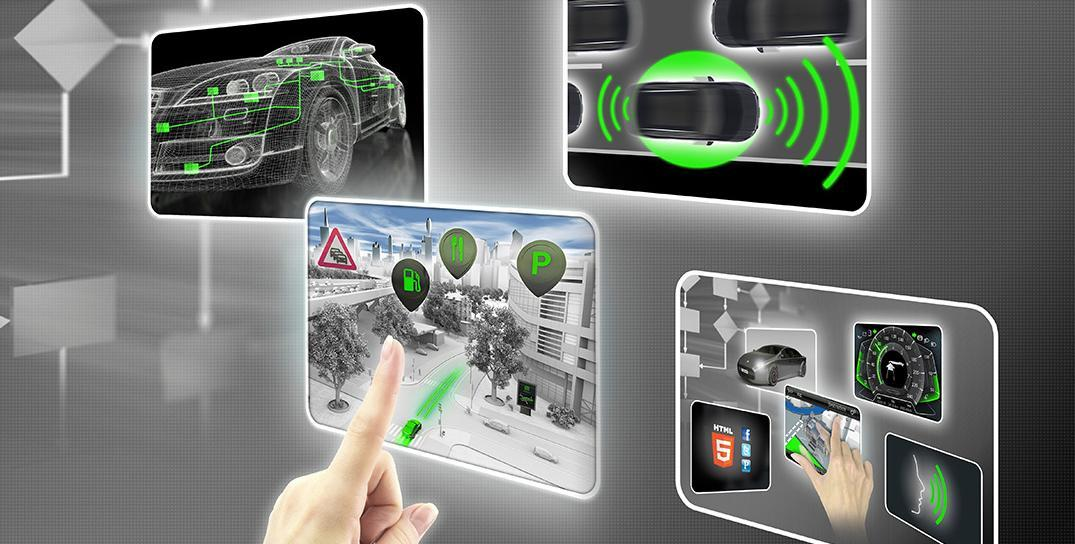
\includegraphics[width=\linewidth]{title_page_figure}

\end{center}

\begin{center}
\vspace{2.2cm}
{\Large{Author:}}
\vspace{0.2cm}

{\Large{\Author}}

\vspace{1.2cm}
{\normalsize{\today}}
\end{center}

% restore baselineskip
\setlength{\baselineskip}{\tmpbaselineskip}
\setlength{\parindent}{\tmpparindent}

% back to normal geometry
\restoregeometry
